\documentclass[final,5p,times,twocolumn]{elsarticle}
%DIF LATEXDIFF DIFFERENCE FILE
%DIF DEL DentalClaw_main                Sat Aug 15 00:53:03 2026
%DIF ADD DentalClaw_main_short_v3.tex   Sat Aug 15 00:27:17 2026
\usepackage{caption}
\usepackage{amssymb}
\usepackage{amsmath}
\usepackage{multirow}
\usepackage{booktabs}
\usepackage{stfloats}
\usepackage{subcaption}
\usepackage{threeparttable}
\usepackage{graphicx}
\usepackage{array}
\usepackage{pifont}
\usepackage{tabularx}
\usepackage[hyphens]{url}
\usepackage[colorlinks,breaklinks]{hyperref}
\usepackage{tikz}
\usepackage{placeins}
\usepackage{enumitem}
%DIF 19d19
%DIF < 
%DIF -------
\newcommand{\cmark}{\ding{51}}
%DIF 21d20
%DIF < 
%DIF -------
\usetikzlibrary{shapes, arrows.meta, positioning, fit, calc}
\usepackage{rotating}
%DIF PREAMBLE EXTENSION ADDED BY LATEXDIFF
%DIF UNDERLINE PREAMBLE %DIF PREAMBLE
\RequirePackage[normalem]{ulem} %DIF PREAMBLE
\RequirePackage{color}\definecolor{RED}{rgb}{1,0,0}\definecolor{BLUE}{rgb}{0,0,1} %DIF PREAMBLE
\providecommand{\DIFaddtex}[1]{{\protect\color{blue}\uwave{#1}}} %DIF PREAMBLE
\providecommand{\DIFdeltex}[1]{{\protect\color{red}\sout{#1}}}                      %DIF PREAMBLE
%DIF SAFE PREAMBLE %DIF PREAMBLE
\providecommand{\DIFaddbegin}{} %DIF PREAMBLE
\providecommand{\DIFaddend}{} %DIF PREAMBLE
\providecommand{\DIFdelbegin}{} %DIF PREAMBLE
\providecommand{\DIFdelend}{} %DIF PREAMBLE
\providecommand{\DIFmodbegin}{} %DIF PREAMBLE
\providecommand{\DIFmodend}{} %DIF PREAMBLE
%DIF FLOATSAFE PREAMBLE %DIF PREAMBLE
\providecommand{\DIFaddFL}[1]{\DIFadd{#1}} %DIF PREAMBLE
\providecommand{\DIFdelFL}[1]{\DIFdel{#1}} %DIF PREAMBLE
\providecommand{\DIFaddbeginFL}{} %DIF PREAMBLE
\providecommand{\DIFaddendFL}{} %DIF PREAMBLE
\providecommand{\DIFdelbeginFL}{} %DIF PREAMBLE
\providecommand{\DIFdelendFL}{} %DIF PREAMBLE
%DIF HYPERREF PREAMBLE %DIF PREAMBLE
\providecommand{\DIFadd}[1]{\texorpdfstring{\DIFaddtex{#1}}{#1}} %DIF PREAMBLE
\providecommand{\DIFdel}[1]{\texorpdfstring{\DIFdeltex{#1}}{}} %DIF PREAMBLE
\newcommand{\DIFscaledelfig}{0.5}
%DIF HIGHLIGHTGRAPHICS PREAMBLE %DIF PREAMBLE
\RequirePackage{settobox} %DIF PREAMBLE
\RequirePackage{letltxmacro} %DIF PREAMBLE
\newsavebox{\DIFdelgraphicsbox} %DIF PREAMBLE
\newlength{\DIFdelgraphicswidth} %DIF PREAMBLE
\newlength{\DIFdelgraphicsheight} %DIF PREAMBLE
% store original definition of \includegraphics %DIF PREAMBLE
\LetLtxMacro{\DIFOincludegraphics}{\includegraphics} %DIF PREAMBLE
\newcommand{\DIFaddincludegraphics}[2][]{{\color{blue}\fbox{\DIFOincludegraphics[#1]{#2}}}} %DIF PREAMBLE
\newcommand{\DIFdelincludegraphics}[2][]{% %DIF PREAMBLE
\sbox{\DIFdelgraphicsbox}{\DIFOincludegraphics[#1]{#2}}% %DIF PREAMBLE
\settoboxwidth{\DIFdelgraphicswidth}{\DIFdelgraphicsbox} %DIF PREAMBLE
\settoboxtotalheight{\DIFdelgraphicsheight}{\DIFdelgraphicsbox} %DIF PREAMBLE
\scalebox{\DIFscaledelfig}{% %DIF PREAMBLE
\parbox[b]{\DIFdelgraphicswidth}{\usebox{\DIFdelgraphicsbox}\\[-\baselineskip] \rule{\DIFdelgraphicswidth}{0em}}\llap{\resizebox{\DIFdelgraphicswidth}{\DIFdelgraphicsheight}{% %DIF PREAMBLE
\setlength{\unitlength}{\DIFdelgraphicswidth}% %DIF PREAMBLE
\begin{picture}(1,1)% %DIF PREAMBLE
\thicklines\linethickness{2pt} %DIF PREAMBLE
{\color[rgb]{1,0,0}\put(0,0){\framebox(1,1){}}}% %DIF PREAMBLE
{\color[rgb]{1,0,0}\put(0,0){\line( 1,1){1}}}% %DIF PREAMBLE
{\color[rgb]{1,0,0}\put(0,1){\line(1,-1){1}}}% %DIF PREAMBLE
\end{picture}% %DIF PREAMBLE
}\hspace*{3pt}}} %DIF PREAMBLE
} %DIF PREAMBLE
\LetLtxMacro{\DIFOaddbegin}{\DIFaddbegin} %DIF PREAMBLE
\LetLtxMacro{\DIFOaddend}{\DIFaddend} %DIF PREAMBLE
\LetLtxMacro{\DIFOdelbegin}{\DIFdelbegin} %DIF PREAMBLE
\LetLtxMacro{\DIFOdelend}{\DIFdelend} %DIF PREAMBLE
\DeclareRobustCommand{\DIFaddbegin}{\DIFOaddbegin \let\includegraphics\DIFaddincludegraphics} %DIF PREAMBLE
\DeclareRobustCommand{\DIFaddend}{\DIFOaddend \let\includegraphics\DIFOincludegraphics} %DIF PREAMBLE
\DeclareRobustCommand{\DIFdelbegin}{\DIFOdelbegin \let\includegraphics\DIFdelincludegraphics} %DIF PREAMBLE
\DeclareRobustCommand{\DIFdelend}{\DIFOaddend \let\includegraphics\DIFOincludegraphics} %DIF PREAMBLE
\LetLtxMacro{\DIFOaddbeginFL}{\DIFaddbeginFL} %DIF PREAMBLE
\LetLtxMacro{\DIFOaddendFL}{\DIFaddendFL} %DIF PREAMBLE
\LetLtxMacro{\DIFOdelbeginFL}{\DIFdelbeginFL} %DIF PREAMBLE
\LetLtxMacro{\DIFOdelendFL}{\DIFdelendFL} %DIF PREAMBLE
\DeclareRobustCommand{\DIFaddbeginFL}{\DIFOaddbeginFL \let\includegraphics\DIFaddincludegraphics} %DIF PREAMBLE
\DeclareRobustCommand{\DIFaddendFL}{\DIFOaddendFL \let\includegraphics\DIFOincludegraphics} %DIF PREAMBLE
\DeclareRobustCommand{\DIFdelbeginFL}{\DIFOdelbeginFL \let\includegraphics\DIFdelincludegraphics} %DIF PREAMBLE
\DeclareRobustCommand{\DIFdelendFL}{\DIFOaddendFL \let\includegraphics\DIFOincludegraphics} %DIF PREAMBLE
%DIF LISTINGS PREAMBLE %DIF PREAMBLE
\RequirePackage{listings} %DIF PREAMBLE
\RequirePackage{color} %DIF PREAMBLE
\lstdefinelanguage{DIFcode}{ %DIF PREAMBLE
%DIF DIFCODE_UNDERLINE %DIF PREAMBLE
  moredelim=[il][\color{red}\sout]{\%DIF\ <\ }, %DIF PREAMBLE
  moredelim=[il][\color{blue}\uwave]{\%DIF\ >\ } %DIF PREAMBLE
} %DIF PREAMBLE
\lstdefinestyle{DIFverbatimstyle}{ %DIF PREAMBLE
	language=DIFcode, %DIF PREAMBLE
	basicstyle=\ttfamily, %DIF PREAMBLE
	columns=fullflexible, %DIF PREAMBLE
	keepspaces=true %DIF PREAMBLE
} %DIF PREAMBLE
\lstnewenvironment{DIFverbatim}{\lstset{style=DIFverbatimstyle}}{} %DIF PREAMBLE
\lstnewenvironment{DIFverbatim*}{\lstset{style=DIFverbatimstyle,showspaces=true}}{} %DIF PREAMBLE
%DIF END PREAMBLE EXTENSION ADDED BY LATEXDIFF

\begin{document}
\begin{frontmatter}

\title{DentalClaw: A Modular Workflow Platform for Standardized and Auditable Dental Imaging AI Experiments}

\begin{abstract}
\textit{Objectives:} Dental imaging artificial intelligence (AI) research increasingly depends on coordinated steps including data curation, preprocessing, model configuration, evaluation, and structured reporting. In practice, these tasks are often fragmented across scripts and manual procedures, making dental AI studies difficult to reproduce and review. This study evaluated DentalClaw, a natural-language-driven workflow platform that converts user intent into executable and auditable dental imaging AI pipelines.\\
\textit{Methods:} DentalClaw was implemented as a modular platform integrating intent parsing, method selection, dataset auditing, model execution, evaluation, and report generation. The system was assessed on representative 2D panoramic radiograph segmentation and 3D cone-beam computed tomography (CBCT) segmentation tasks, and its decision layer was evaluated across 11 representative natural-language intents spanning executable, ambiguous, boundary, and out-of-scope cases.\\
\textit{Results:} DentalClaw completed end-to-end workflows for both representative public dental imaging tasks and generated standardized outputs including split files, prediction results, evaluation tables, and review-oriented reports. Compared with manually assembled script-based workflows, the platform reduced coordination effort during dataset preparation and result organization while preserving a consistent execution trace. The intent-to-workflow evaluation achieved a weighted score of 0.977, and no incorrect workflow was silently executed.\\
\textit{Conclusions:} DentalClaw demonstrated feasibility for translating natural-language research intent into auditable and executable dental imaging AI workflows under representative settings. The study supports the platform as a workflow orchestration and validation framework rather than as a new segmentation model or as a standalone clinical decision-support system.\\
\textit{Clinical Significance:} By standardizing workflow execution and traceability, DentalClaw lowers the technical barrier for dental researchers while preserving a reviewable record of the data, configuration, and outputs associated with dental AI studies.
\end{abstract}

\begin{keyword}
Dental informatics \sep Artificial intelligence \sep Digital dentistry \sep Workflow automation \sep Auditable experiments \sep Cone-beam computed tomography \sep Panoramic radiography
\end{keyword}

\end{frontmatter}

\section{Introduction}

\begin{figure*}[t]
\centering
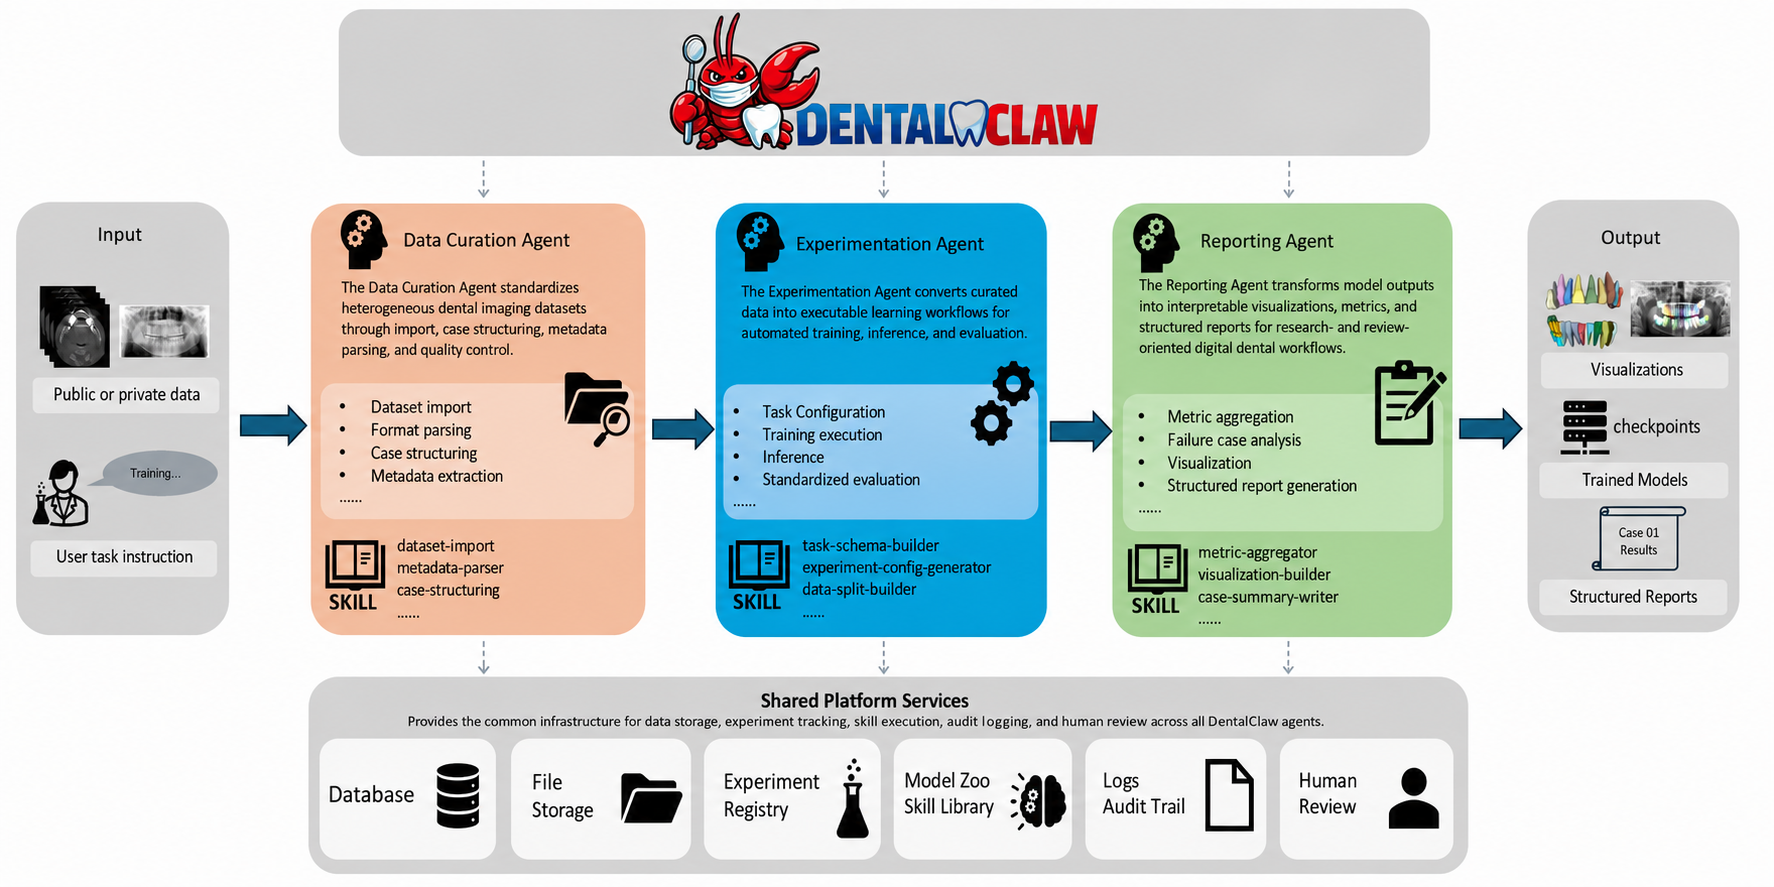
\includegraphics[width=\textwidth]{Multi-agent system architecture of DentalClaw.pdf}
\caption{Overview of the DentalClaw architecture. Heterogeneous dental imaging inputs and user instructions are processed by a central coordinator and routed to specialized data-curation, experimentation, and reporting agents. Shared platform services provide dataset organization, model and skill libraries, audit logs, and human review support.}
\label{fig:system_overview}
\end{figure*}

Dental imaging AI has become increasingly relevant for tooth segmentation, lesion detection, treatment planning support, and image-based diagnosis in digital dentistry~\cite{Horner2012,Kapila2015,Schwendicke2020,Shujaat2021}. In recent years, deep learning methods have shown strong performance in dental radiographs and CBCT analysis; however, the practical challenge of translating a study idea into a reproducible workflow remains substantial. In many real-world projects, the bottleneck is not the absence of a capable model but the fragmented process of dataset curation, annotation harmonization, preprocessing, model selection, evaluation, and final report generation~\cite{Schwendicke2021Checklist,Polizzi2023,Dot2024DentalSegmentator}. These steps are often implemented as ad hoc scripts or local procedures, which makes results difficult to reproduce, compare, and audit across studies.

This problem is amplified by the heterogeneity of dental imaging data. Panoramic radiographs, periapical images, CBCT volumes, and clinical annotations differ in file format, dimensionality, metadata structure, image quality, and case-level quality-control requirements. Variations in labeling conventions, field-of-view completeness, and patient-level splitting can lead to overly optimistic performance estimates and undermine reproducibility across institutions~\cite{Nemtoi2013,Schwendicke2021Checklist,Polizzi2023}. These issues are especially relevant when clinicians or dental researchers understand the clinical objective but do not have the engineering infrastructure needed to execute the full workflow reliably.

Existing software tools partly address this challenge. General medical imaging frameworks such as nnU-Net and MONAI provide strong model-development primitives~\cite{Isensee2021nnUNet,Fedorov2012Slicer}, while dental-specific tools often target a narrow task or a single modality. DentalClaw addresses a complementary need: it orchestrates the experimental workflow around user intent, converts natural-language requests into candidate executable routes, and records actions in an auditable form. In this sense, the platform is best understood as an orchestration layer rather than as a new segmentation model.

The objective of this study was to assess whether a clinician-facing workflow platform could reduce the technical barrier of dental imaging AI research by transforming natural-language instructions into executable, reviewable, and traceable research pipelines. We evaluated DentalClaw on representative 2D panoramic radiograph segmentation and 3D CBCT segmentation tasks, and we assessed its decision pipeline on 11 representative intents spanning executable, ambiguous, boundary, and out-of-scope cases. This design allows the platform to be judged not only by final segmentation metrics, but also by whether it can correctly map a user request to an appropriate workflow, maintain traceability, and prevent unsupported actions from being silently executed.

\begin{figure*}[b!]
\centering
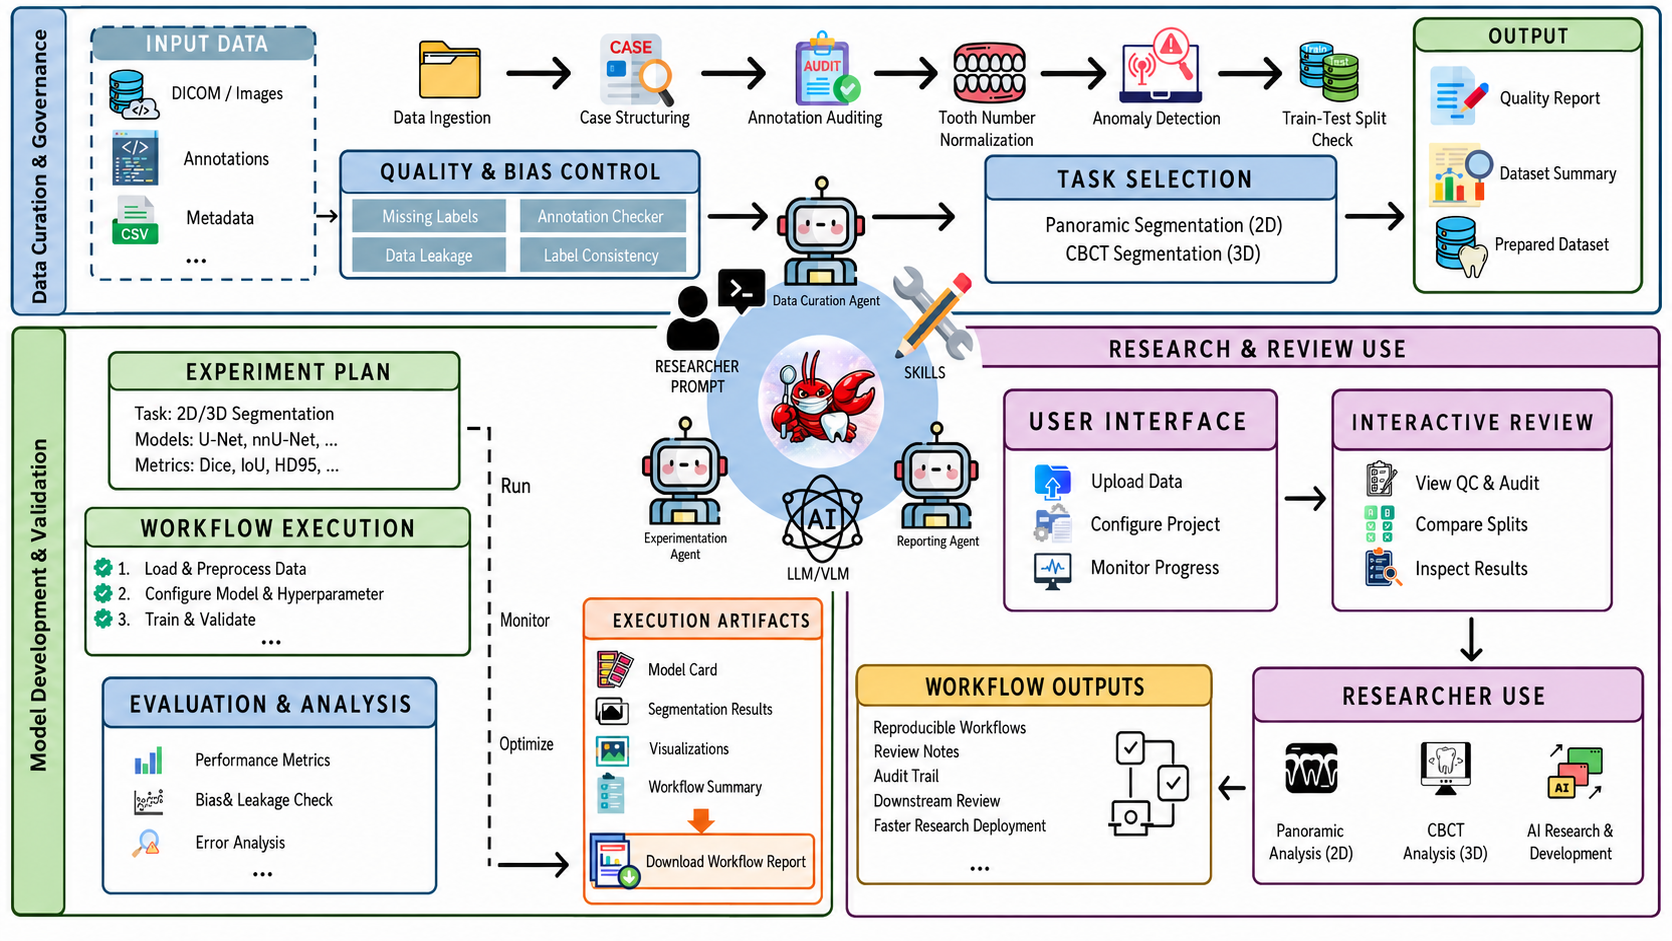
\includegraphics[width=\textwidth]{Overall workflow of DentalClaw.pdf}
\caption{Overall workflow of DentalClaw. User intent is parsed into structured fields, matched against a registry of validated methods, and routed to either an executable path or a human-reviewed external proposal. Deterministic modules perform dataset preparation, model execution, evaluation, and reporting.}
\label{fig:framework}
\end{figure*}

\section{Materials and methods}

\subsection{Study design and platform overview}
DentalClaw was implemented as a modular workflow platform built around OpenClaw~\cite{openclaw}. The system includes a natural-language reasoning layer, an offline method registry, dataset and quality-control modules, task-specific execution routes, and structured reporting. The agent parses a user request into structured fields including dataset, task family, modality, mode, and optional TTA or ensemble flags. It then performs registry lookup and, when necessary, proposal generation. The design is intentionally conservative: unsupported or ambiguous requests are rejected, while external proposals are surfaced for human review instead of being executed automatically.

The execution layer contains deterministic modules for dataset preparation, preprocessing, model training or inference, evaluation, and report generation. Each module stores its configuration, intermediate outputs, and workflow status to preserve traceability. This separation of decision logic from execution logic is central to the platform design: the agent decides which workflow should be attempted, while the deterministic runner executes only the validated route or an approved external proposal.

For the present study, the platform was evaluated on a server equipped with an NVIDIA GeForce RTX 3090 GPU. The decision layer was powered by the OpenClaw runtime, with DeepSeek V4 Pro as the primary reasoning backend. Literature-search support was drawn from Europe PMC and arXiv to provide task-relevant references and alternative method suggestions when no validated route was registered.

\subsection{Agent decision pipeline}
The agent decision pipeline operated in five stages. First, the user's natural-language input was parsed into structured fields such as dataset, task family, modality, mode, and optional TTA or ensemble flags. The system also detected the interface language automatically, supporting both Chinese and English inputs. Second, a task-aware academic search was generated from the parsed intent and queried against Europe PMC and arXiv. Third, the offline method registry was queried to determine whether a validated executable path existed for the requested task. Fourth, the agent synthesized the parsed intent, registry status, search results, and available codebase assets to produce one of three outcomes: \texttt{use\_registry}, \texttt{external\_proposal}, or \texttt{reject}. Fifth, the final plan was serialized in a machine-readable file that recorded the selected method, decision rationale, cited references, prerequisite checks, and whether human review was required before execution.

This plan-based design offers two practical advantages. First, the platform can distinguish between a supported workflow, an external but promising option, and an unsupported request without silent fallback behavior. Second, the record created for each run improves reproducibility and allows downstream auditing of the exact intent, chosen route, and execution parameters.

\subsection{Datasets and representative workflows}
Two public datasets and one private dataset were used for validation. The Tufts Dental Database (TDD)~\cite{panetta2022tufts} was used for 2D panoramic radiograph segmentation. After audit and curation, 968 of 1051 cases were retained for downstream processing. ToothFairy~\cite{ToothFairyDataset1,ToothFairyDataset2,ToothFairyDataset3} was used for 3D CBCT segmentation. Together, these tasks represent two common dental imaging scenarios with different dimensionality, metadata structure, and preprocessing requirements.

A private panoramic dataset was also used for exploratory task extension and quality review. It included 290 images collected during routine clinical care, with annotations for lesion and restoration regions. While this dataset was not the primary focus of the platform validation, it was useful for testing how the system handled additional private, clinically relevant data and how it generated review-oriented outputs around real-world case quality.

\subsection{Workflow execution and quality control}
All datasets were converted to a canonical case-level representation before model execution. Each case record retained image references, annotation files, modality information, and workflow status indicators. Built-in quality-control functions then checked image completeness, annotation integrity, metadata consistency, and train--test leakage risk. For flagged cases, the platform recorded the issue category and handling decision, including normalization, exclusion, or manual review.

After validation, DentalClaw generated a task-specific execution plan specifying preprocessing rules, split assignment, output directories, and evaluation settings. The execution pipeline then invoked the selected model route, generated predictions, computed standard segmentation metrics, and exported structured reports for expert review. This approach helps standardize workflow execution without requiring users to manually coordinate low-level dataset preparation steps.

\subsection{Evaluation protocol}
The evaluation strategy included both workflow-level validation and intent-level decision testing. At the workflow level, DentalClaw was examined for successful completion across 2D panoramic and 3D CBCT segmentation tasks, including dataset preparation, model execution, output generation, and structured reporting. At the decision level, we constructed a six-dimension weighted evaluation framework across 11 representative intents covering standard executable requests, ambiguous requests, boundary cases, and out-of-scope queries. A decision was considered correct only when the selected route matched the intended dataset, task family, modality, and execution mode, or when the request was correctly rejected.

The six dimensions were: planning, QC blocking, intent parsing, external proposal quality, ambiguity handling, and boundary identification. Weighted scoring provided a transparent estimate of how well the platform handled both execution and safety-critical failure modes. In the current study, the overall weighted score was 0.977.

\section{Results}

\subsection{Workflow completion and reproducibility}
\begin{figure*}[!t]
\centering
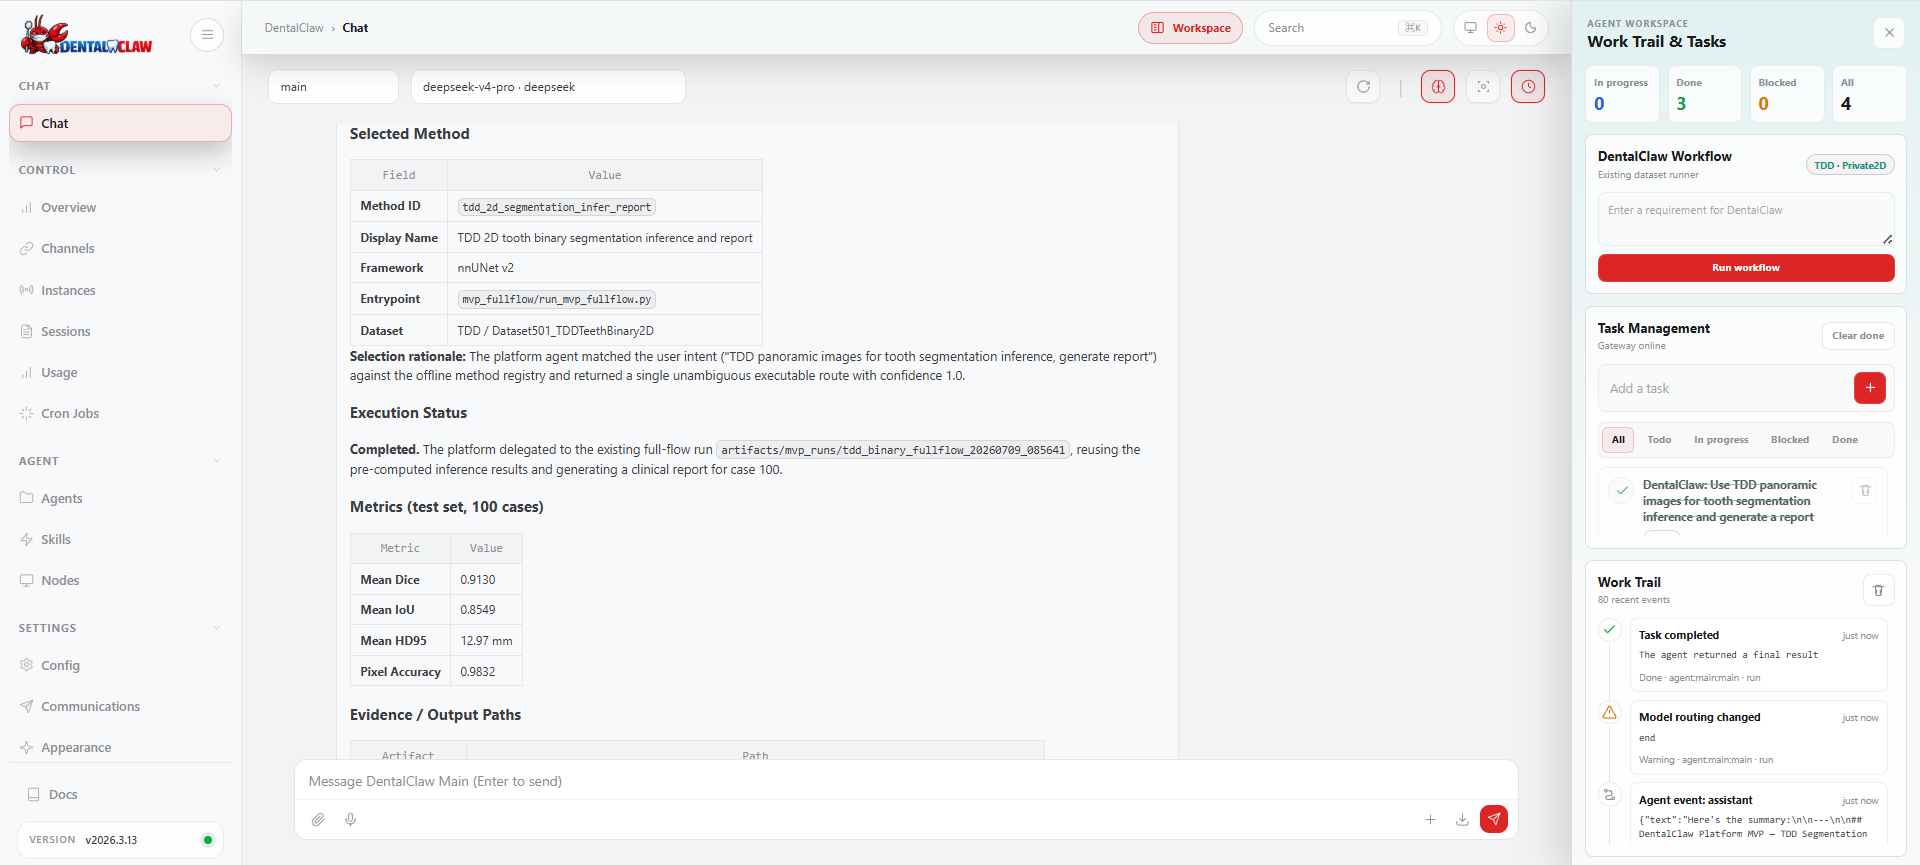
\includegraphics[width=0.95\textwidth]{Complete training.png}
\caption{Front-end workflow trace of DentalClaw showing the agent planning, task scheduling, and report-generation state during a completed run. The interface makes the decision and execution path visible for review and auditability.}
\label{fig:complete_training}
\end{figure*}

DentalClaw completed end-to-end workflows for the representative public datasets used in this study. In the 2D panoramic setting, the platform executed dataset curation, model training, inference, evaluation, and structured reporting. In the 3D CBCT setting, it handled volumetric data with modality-specific preprocessing, multi-model execution, and result aggregation under the same orchestration framework. Across both tasks, the platform generated standardized outputs including manifests, split files, predictions, metrics tables, and review-oriented reports.

This result is important because the two tasks differ substantially in data organization, preprocessing requirements, and execution logic. The 2D workflow centered on panoramic images and tooth-level segmentation, whereas the CBCT workflow involved volumetric data, anatomical complexity, and more demanding multi-model coordination. The fact that the same workflow abstraction handled both settings suggests that DentalClaw provided a consistent execution framework without sacrificing modality-specific adaptation.

Table~\ref{tab:workflow_validation} summarizes workflow-level outcomes and compares them with a manually assembled script baseline. The baseline followed the same predefined task but required substantially more operator coordination. DentalClaw reduced time spent on dataset preparation and result organization while preserving a consistent execution record for downstream review.

\begin{table*}[!t]
\centering
\small
\setlength{\tabcolsep}{4pt}
\renewcommand{\arraystretch}{1.12}
\caption{End-to-end workflow completion and coordination efficiency. The manual baseline used the same workflow without additional hyperparameter tuning or model selection.}
\label{tab:workflow_validation}
\begin{threeparttable}
\begin{tabularx}{\textwidth}{>{\raggedright\arraybackslash}p{2.3cm}>{\centering\arraybackslash}p{1.6cm}>{\raggedright\arraybackslash}p{3.0cm}>{\centering\arraybackslash}p{1.4cm}>{\raggedright\arraybackslash}X>{\raggedright\arraybackslash}X}
\toprule
Task & Cases input / eligible & Main preparation findings & Completion & DentalClaw & Manual workflow \\
\midrule
Panoramic segmentation & 1051 / 968 & Missing masks; image--label mismatch & Completed & audit+prep 14 min; train 6 h 52 min; infer+eval+report 31 min; outputs: manifest, split file, predictions, metrics, report & audit+prep 3 h 26 min; train 6 h 58 min; infer+eval+organization 2 h 18 min; outputs: ad hoc logs and files \\
\addlinespace
CBCT segmentation & 63 / 43 & Metal artifacts; FOV anomalies; inconsistent volume usability & Completed & audit+prep 21 min; train 19 h 36 min; infer+eval+report 1 h 44 min; outputs: manifest, split file, volumes, metrics, report & audit+prep 6 h 12 min; train 19 h 49 min; infer+eval+organization 3 h 11 min; outputs: ad hoc logs and files \\
\bottomrule
\end{tabularx}
\end{threeparttable}
\end{table*}

\subsection{Intent-to-workflow decision accuracy}
To assess the agent's decision capability, we evaluated the full pipeline across 11 representative natural-language requests. The results are summarized in Table~\ref{tab:intent_results}. The platform correctly selected the registered method for all five standard executable intents, correctly rejected both trap requests, and correctly handled ambiguous or incomplete requests without silently executing an incorrect workflow. For boundary cases without a registered method, the agent proposed external solutions but explicitly flagged them for human review.

\begin{table*}[!t]
\centering
\caption{Intent-to-workflow decision accuracy across 11 representative intents.}
\label{tab:intent_results}
\footnotesize
\begin{tabular}{@{}c p{5.4cm} p{2.1cm} c p{4.0cm}@{}}
\hline
\# & \textbf{Intent} & \textbf{Category} & \textbf{Score} & \textbf{Method selected} \\
\hline
1 & TDD panoramic tooth segmentation inference & standard & 1.00 & \texttt{tdd\_2d\_seg\_infer\_report} \\
2 & TDD panoramic super-resolution enhancement & standard & 1.00 & \texttt{dental\_2d\_super\_resolution} \\
3 & ToothFairy3 CBCT 3D tooth segmentation & standard & 1.00 & \texttt{toothfairy3\_3d\_seg\_...} \\
4 & Private dental data segmentation training & standard & 1.00 & \texttt{private\_2d\_segmentation\_train} \\
5 & Dental anomaly detection (panoramic) & standard & 1.00 & \texttt{dental\_anomaly\_detection} \\
6 & ``Build a model with TDD'' (vague task) & ambiguous & 1.00 & \texttt{platform\_clarification} \\
7 & ``Write a dental AI paper'' (non-CV) & trap & 1.00 & Rejected (\texttt{supported=false}) \\
8 & ``Video action recognition'' (non-dental) & trap & 1.00 & Rejected (\texttt{supported=false}) \\
9 & Inference on private data (no task specified) & boundary & 1.00 & \texttt{platform\_clarification} \\
10 & TDD tooth segmentation training & boundary & 0.98 & \texttt{agent\_external\_suggestion} \\
11 & TDD bbox tooth detection training & boundary & 0.98 & \texttt{agent\_external\_suggestion} \\
\hline
\multicolumn{5}{@{}c@{}}{Weighted average: \textbf{0.977} \quad (all $\ge$ 0.70 threshold)} \\
\end{tabular}
\end{table*}

The weighted overall score of 0.977 indicates that the platform performed strongly on both supported tasks and safety-critical rejection behaviors. This is a meaningful result in the context of dental AI workflow automation: the platform should not silently execute unsupported tasks. A method that is conservative but correct is preferable to one that appears more flexible but executes the wrong route.

\subsection{Structured reporting and review-oriented outputs}
Beyond task execution, DentalClaw generated structured outputs designed to support expert review and workflow traceability. For each validated task, the platform exported workflow metadata, preparation summaries, model configuration records, quantitative evaluation tables, prediction files, and case-level notes in a consistent format. This output layer was designed to go beyond isolated model artifacts and provide a review-friendly summary of what was run, on which data, and under which settings.

A representative report generated by DentalClaw is shown in Fig.~\ref{fig:report_figure}. The report organized information into three layers: workflow-level metadata, quantitative performance summaries, and case-level notes flagging review-relevant findings. This design is particularly relevant for dental AI research, where transparency of data handling and procedural traceability may be as important as the final numerical metrics.

\begin{figure*}[htbp!]
\centering
\includegraphics[width=0.95\textwidth]{report_figure.png}
\caption{A representative structured report generated by DentalClaw. The report integrates workflow metadata, quantitative performance summaries, and case-level visual review panels to improve auditability and clinician-facing interpretation.}
\label{fig:report_figure}
\vspace{1em}
\end{figure*}

\section{Discussion}
DentalClaw should be interpreted as a workflow infrastructure layer rather than as a new segmentation model. Frameworks such as nnU-Net and MONAI provide strong building blocks for model training and image processing, while DentalClaw addresses a different problem: translating a natural-language research intent into a guided, auditable, and executable workflow. This distinction is important because real-world dental AI research usually fails less from a lack of capable models than from the difficulty of coordinating data preparation, task selection, validation, and reporting consistently.

The findings of this study support the feasibility of this approach. DentalClaw completed representative 2D and 3D workflows, reduced manual coordination, and generated structured review-oriented outputs. The decision pipeline also showed strong reliability on the tested intent set, with a weighted score of 0.977. These results suggest that the platform can route a natural-language request to a supported workflow or reject an unsupported one without silently executing the wrong pipeline.

Several limitations remain. The evaluation was performed on representative rather than exhaustive tasks, and the current study did not include a formal usability experiment with clinicians or dental researchers. In addition, the platform intentionally adopts a conservative external-proposal policy: external routes are surfaced for explicit approval before execution. This design protects against silent execution of incorrect or hallucinated workflows, but it also limits automation when a task falls outside the validated registry. Future work should expand the task set, conduct user-facing validation, and benchmark broader multimodal and clinically relevant scenarios.

\section{Conclusion}
This study evaluated DentalClaw as an intent-driven workflow platform for standardized and auditable dental imaging AI research. Under representative 2D and 3D tasks, the system converted natural-language instructions into executable workflows, tracked workflow state in a reviewable form, and generated structured outputs for dataset preparation, model execution, evaluation, and reporting. The findings support the feasibility of this workflow-oriented approach in dental imaging AI while clarifying that the current contribution should be interpreted as a platform validation study rather than as a general-purpose clinical decision-support tool or a new segmentation architecture.

\newpage
\footnotesize
\bibliographystyle{elsarticle-num}
\bibliography{cas-refs}

\end{document}
